\section{Bluetooth}
\subsection{Histoire}
\begin{frame}

\begin{minipage}[t]{0.25\linewidth}

\begin{figure}
\includegraphics[height=2.5cm]{bt_logo.png}
\caption{Logo Bluetooth}
\end{figure}

\end{minipage}\hfill
\begin{minipage}[t]{0.72\linewidth}
\begin{block}{Historique}
\begin{itemize}
	\item 1994 : Création ( Ericsson )
	\item 1998 : SIG (Ericsson, Intel, Nokia, Toshiba)
	\item 1999 : v1.0
	\item 2010 : v4.0 Low Energy
	\item 2014 : v4.2
\end{itemize}
\end{block}
\begin{block}{Caractéristiques physiques}
\begin{itemize}
\item 2.4 GHz
\item 10m ( class 2 )
\item Max 24Mb/s
\item 79 cannaux, AFH
\end{itemize}
\end{block}

\end{minipage}
\end{frame}

% Présenter des schémas
\subsection{Architecture logique}

\begin{frame}

\begin{minipage}[t]{0.45\linewidth}

\begin{figure}
\vspace{0.5cm}
\includegraphics[height=5.5cm]{arch_core.png}
\caption{Bluetooth core}
\end{figure}

\end{minipage}
\begin{minipage}[t]{0.52\linewidth}
\begin{block}{Host}
\begin{itemize}
	\item Logique Métier
	\item Scheduling
	\item Buffering
	\item QoS
\end{itemize}
\end{block}

\begin{block}{Controller}
\begin{itemize}
	\item Connexion
	\item Découverte
	\item Sécurité
	\item QoS
\end{itemize}
\end{block}


\end{minipage}
\end{frame}

\begin{frame}
	\begin{figure}
		\includegraphics[height=6cm]{arch_log_hci.png}
		\caption{Host to Controller Interface}
	\end{figure}
\end{frame}

\begin{frame}
\begin{figure}
\includegraphics[height=6cm]{arch_log_l2cap.png}
\caption{Logical Link Control and Adaptation Protocol}
\end{figure}
\end{frame}

\begin{frame}
\begin{figure}
\includegraphics[height=6cm]{arch_log_all.png}
\caption{Profils}
\end{figure}
\end{frame}

\subsection{Appairage}
\begin{frame}
Appairage
\end{frame}

\subsection{Découverte de services}
\begin{frame}
SDPA
\end{frame}
